\ifx\wholebook\relax \else
% ------------------------ 

\documentclass{article}
%------------------- Other types of document example ------------------------
%
%\documentclass[twocolumn]{IEEEtran-new}
%\documentclass[12pt,twoside,draft]{IEEEtran}
%\documentstyle[9pt,twocolumn,technote,twoside]{IEEEtran}
%
%-----------------------------------------------------------------------------
%%
% loading packages
%
\newif\ifpdf
\ifx\pdfoutput\undefined % We're not running pdftex
  \pdffalse
\else
  \pdftrue
\fi
%
%
\ifpdf
  \RequirePackage[pdftex,%
            CJKbookmarks,%
       bookmarksnumbered,%
              colorlinks,%
          linkcolor=blue,%
              hyperindex,%
        plainpages=false,%
       pdfstartview=FitH]{hyperref}
\else
  \RequirePackage[dvipdfm,%
             CJKbookmarks,%
        bookmarksnumbered,%
               colorlinks,%
           linkcolor=blue,%
               hyperindex,%
         plainpages=false,%
        pdfstartview=FitH]{hyperref}
  \AtBeginDvi{\special{pdf:tounicode GBK-EUC-UCS2}} % GBK -> Unicode
\fi
\usepackage{hyperref}

% other packages
%-----------------------------------------------------------------------------
\usepackage{graphicx, color}
\usepackage{CJK}
%
% for programming 
%
\usepackage{verbatim}
\usepackage{listings}


\lstdefinelanguage{Smalltalk}{
  morekeywords={self,super,true,false,nil,thisContext}, % This is overkill
  morestring=[d]',
  morecomment=[s]{"}{"},
  alsoletter={\#:},
  escapechar={!},
  literate=
    {BANG}{!}1
    {UNDERSCORE}{\_}1
    {\\st}{Smalltalk}9 % convenience -- in case \st occurs in code
    % {'}{{\textquotesingle}}1 % replaced by upquote=true in \lstset
    {_}{{$\leftarrow$}}1
    {>>>}{{\sep}}1
    {^}{{$\uparrow$}}1
    {~}{{$\sim$}}1
    {-}{{\sf -\hspace{-0.13em}-}}1  % the goal is to make - the same width as +
    %{+}{\raisebox{0.08ex}{+}}1		% and to raise + off the baseline to match -
    {-->}{{\quad$\longrightarrow$\quad}}3
	, % Don't forget the comma at the end!
  tabsize=2
}[keywords,comments,strings]

\lstloadlanguages{C++, Lisp, Smalltalk}

% ======================================================================

\def\BibTeX{{\rm B\kern-.05em{\sc i\kern-.025em b}\kern-.08em
    T\kern-.1667em\lower.7ex\hbox{E}\kern-.125emX}}

\newtheorem{theorem}{Theorem}

%
% mathematics
%
\newcommand{\be}{\begin{equation}}
\newcommand{\ee}{\end{equation}}
\newcommand{\bmat}[1]{\left( \begin{array}{#1} }
\newcommand{\emat}{\end{array} \right) }
\newcommand{\VEC}[1]{\mbox{\boldmath $#1$}}

% numbered equation array
\newcommand{\bea}{\begin{eqnarray}}
\newcommand{\eea}{\end{eqnarray}}

% equation array not numbered
\newcommand{\bean}{\begin{eqnarray*}}
\newcommand{\eean}{\end{eqnarray*}}

\RequirePackage{CJK,CJKnumb,CJKulem,CJKpunct}
% we use CJK as default environment
\AtBeginDocument{\begin{CJK*}{GBK}{song}\CJKtilde\CJKindent\CJKcaption{GB}}
\AtEndDocument{\clearpage\end{CJK*}}

%
% loading packages
%
\newif\ifpdf
\ifx\pdfoutput\undefined % We're not running pdftex
  \pdffalse
\else
  \pdftrue
\fi
%
%
\ifpdf
  \RequirePackage[pdftex,%
       bookmarksnumbered,%
              colorlinks,%
          linkcolor=blue,%
              hyperindex,%
        plainpages=false,%
       pdfstartview=FitH]{hyperref}
\else
  \RequirePackage[dvipdfm,%
        bookmarksnumbered,%
               colorlinks,%
           linkcolor=blue,%
               hyperindex,%
         plainpages=false,%
        pdfstartview=FitH]{hyperref}
\fi
\usepackage{hyperref}

% other packages
%-----------------------------------------------------------------------------
\usepackage{graphicx, color}
%
% for programming 
%
\usepackage{verbatim}
\usepackage{listings}
\usepackage{algorithmic} %for pseudocode
\usepackage{algorithm}


\lstdefinelanguage{Smalltalk}{
  morekeywords={self,super,true,false,nil,thisContext}, % This is overkill
  morestring=[d]',
  morecomment=[s]{"}{"},
  alsoletter={\#:},
  escapechar={!},
  literate=
    {BANG}{!}1
    {UNDERSCORE}{\_}1
    {\\st}{Smalltalk}9 % convenience -- in case \st occurs in code
    % {'}{{\textquotesingle}}1 % replaced by upquote=true in \lstset
    {_}{{$\leftarrow$}}1
    {>>>}{{\sep}}1
    {^}{{$\uparrow$}}1
    {~}{{$\sim$}}1
    {-}{{\sf -\hspace{-0.13em}-}}1  % the goal is to make - the same width as +
    %{+}{\raisebox{0.08ex}{+}}1		% and to raise + off the baseline to match -
    {-->}{{\quad$\longrightarrow$\quad}}3
	, % Don't forget the comma at the end!
  tabsize=2
}[keywords,comments,strings]

\lstloadlanguages{C++, Lisp, Haskell, Python, Smalltalk}

% ======================================================================

\def\BibTeX{{\rm B\kern-.05em{\sc i\kern-.025em b}\kern-.08em
    T\kern-.1667em\lower.7ex\hbox{E}\kern-.125emX}}

\newtheorem{theorem}{Theorem}

%
% mathematics
%
\newcommand{\be}{\begin{equation}}
\newcommand{\ee}{\end{equation}}
\newcommand{\bmat}[1]{\left( \begin{array}{#1} }
\newcommand{\emat}{\end{array} \right) }
\newcommand{\VEC}[1]{\mbox{\boldmath $#1$}}

% numbered equation array
\newcommand{\bea}{\begin{eqnarray}}
\newcommand{\eea}{\end{eqnarray}}

% equation array not numbered
\newcommand{\bean}{\begin{eqnarray*}}
\newcommand{\eean}{\end{eqnarray*}}




\setcounter{page}{1}

\begin{document}

\fi
%--------------------------

% ================================================================
%                 COVER PAGE
% ================================================================

\title{Queue, not so simple as it was thought}

\author{Liu~Xinyu
\thanks{{\bfseries Liu Xinyu } \newline
  Email: liuxinyu95@gmail.com \newline}
  }

\markboth{Queue}{AlgoXY}

\maketitle

\ifx\wholebook\relax
\chapter{Queue, not so simple as it was thought}
\numberwithin{Exercise}{chapter}
\fi

% ================================================================
%                 Introduction
% ================================================================
\section{Introduction}
\label{introduction}
It seems that queues are relative simple. A queue provides FIFO (first-in,
first-out) data manipulation support. There are many options to 
realize queue includes singly linked-list, doubly linked-list,
circular buffer etc. However, we'll show that it's not so easy to 
realize queue in purely funcitonal settings if it must satisfy
abstract queue properties.

In this chapter, we'll present several different approaches to 
implement queue. And in next chapter, we'll explain how to realize
sequence.

A queue is a FIFO data structure satisfies the following performance
constraints.

\begin{itemize}
\item Element can be added to the tail of the queue in $O(1)$ constant time;
\item Element can be removed from the head of the queue in $O(1)$ constant time.
\end{itemize}

These two properties must be satisfied. And it's common to add some extra
targets, such as dynamic memory allocation etc.

Of course such abstract queue interface can be implemented with 
doubly-linked list trivially. But this is a overkill solution. 
We can even implement imperative queue with singly linked-list or
plained array. However, our main question here is about how to realize
a purely functional queue as well?

We'll first review the typical queue solution which is realized by
singlely linked-list and circular buffer in first section; Then we
give a simple and straightforward functional solution in the second
section. While the performance is ensured in terms of amortized
constant time, we need find realtime solution (or worst-time solution)
for some special case. Such solution will be described in the third
and the fourth section. Finally, we'll show a very simple real time
queue which depends on lazy evaluation.

% ================================================================
%                 Imperative queue
% ================================================================
\section{Queue by linked-list and circular buffer}

\subsection{Singly linked-list solution}
\index{Queue!Singly linked-list}

Queue can be implemented with singly linked-list. It's easy to add 
and remove element at the front end of a linked-list in $O(1)$ time. 
However, in
order to keep the FIFO order, if we execute one operation on head,
we must perform the inverse operation on tail.

For plain singly linked-list, we must traverse the whole list before
adding or removing. Travering is bound to $O(N)$ time, 
where $N$ is the length of the list. This doesn't match the abstract
queue properties.

The solution is to use an extra record to store the tail of the linked-list.
A sentinel is often used to simplify the boundery handling. The 
following ANSI C \footnote{It's possible to parameterize the type of the key
with C++ template. ANSI C is used here for illustration purpose.} 
code defines a queue realized by linked-list.

\lstset{language=C}
\begin{lstlisting}
typedef int Key;

struct Node{
  Key key;
  struct Node* next;
};

struct Queue{
  struct Node *head, *tail;
};
\end{lstlisting}

Figure \ref{fig:empty-list} illustrates an empty list. Both head
and tail point to the sentinel NIL node.

\begin{figure}[htbp]
  \centering
  \includegraphics[scale=1.0]{img/empty-list.ps}
  \caption{The empty queue, both head and tail point to sentinel node.} \label{fig:empty-list}
\end{figure}

We summarize the abstract queue interface as the following.

\begin{algorithmic}
\Function{Empty}{}
  \Comment{Create an empty queue}
\EndFunction
\Function{Empty?}{$Q$}
  \Comment{Test if $Q$ is empty}
\EndFunction
\Function{Enqueue}{$Q, x$}
  \Comment{Add a new element $x$ to queue $Q$}
\EndFunction
\Function{Dequeue}{$Q$}
  \Comment{Remove element from queue $Q$}
\EndFunction
\Function{Head}{$Q$}
  \Comment{get the next element in queue $Q$ in FIFO order}
\EndFunction
\end{algorithmic}

Note the difference between \textproc{Dequeue} and \textproc{Head}.
\textproc{Head} only retrieve next element in FIFO order without removing
it, while \textproc{Dequeue} performs removing.

To ensure the constant time \textproc{Enqueue} and \textproc{Dequeue},
we add new element to head and remove element from tail.\footnote{It's possible
to add new element to the tail, while remove element from head, but the 
operatoins are more complex than this approach.}

\begin{algorithmic}
\Function{Enqueue}{$Q, x$}
  \State $p \gets $ \Call{Create-New-Node}{}
  \State \Call{Key}{$p$} $\gets x$
  \State \Call{Next}{$p$} $\gets NIL$
  \State \textproc{Next}(\Call{Tail}{$Q$}) $\gets p$
  \State \Call{Tail}{$Q$} $\gets p$
\EndFunction
\end{algorithmic}

Note that, as we use the sentinel node, there are at least one node, the
sentinel in the queue. That's why we needn't check the validation of
of the tail before we append the new created node $p$ to it.

\begin{algorithmic}
\Function{Dequeue}{$Q$}
  \State $x \gets $ \Call{Head}{$Q$}
  \State \textproc{Next}(\Call{Head}{$Q$}) $\gets$ \Call{Next}{$x$}
  \If{$x = $ \Call{Tail}{$Q$}} \Comment{$Q$ gets empty}
    \State \Call{Tail}{$Q$} $\gets$ \Call{Head}{$Q$}
  \EndIf
  \State \Return \Call{Key}{$x$}
\EndFunction
\end{algorithmic}

As we always put the sentinel node in front of all the other nodes,
function \textproc{Head} actually returns the next node to the sentinel.

Figure \ref{fig:list-queue} illustrates \textproc{Enqueue} and \textproc{Dequeue} process with sentinel node.

\begin{figure}[htbp]
 \centering
 \subfloat[Before \textproc{Enqueue} $x$ to queue]{\includegraphics[scale=0.8]{img/enq-list-before.ps}} \\
 \subfloat[After \textproc{Enqueue} $x$ to queue]{\includegraphics[scale=0.8]{img/enq-list-after.ps}} \\
 \subfloat[Before \textproc{Dequeue} $x$ to queue]{\includegraphics[scale=0.8]{img/deq-list-before.ps}} \\
 \subfloat[After \textproc{Dequeue} $x$ to queue]{\includegraphics[scale=0.8]{img/deq-list-after.ps}} \\
 \caption{\textproc{Enqueue} and \textproc{Dequeue} to linked-list queue.} \label{fig:list-queue}
\end{figure}

Translating the pseudo code to ANSI C program yields the below code.

\begin{lstlisting}
struct Queue* enqueue(struct Queue* q, Key x){
  struct Node* p = (struct Node*)malloc(sizeof(struct Node));
  p->key = x;
  p->next = NULL;
  q->tail->next = p;
  q->tail = p;
  return q;
}

Key dequeue(struct Queue* q){
  struct Node* p = head(q); /*gets the node next to sentinel*/
  Key x = key(p);
  q->head->next = p->next;
  if(q->tail == p)
    q->tail = q->head;
  free(p);
  return x;
}
\end{lstlisting}

This solution is simple and robust. It's easy to extend this solution 
even to the concurrent environment (e.g. multi-cores). We can assign
a lock to the head and use another lock to the tail. The sentinel 
helps us from being dead-locked due to the empty case \cite{PODC96} \cite{SutterDDJ}.

\begin{Exercise}
\begin{itemize}
\item Realize the \textproc{Empty?} and \textproc{Head} algorithms
for linked-list queue.

\item Implement the singly linked-list queue in your favorate imperative 
programming language. Note that you need provide functions to initialze
and destroy the queue.
\end{itemize}
\end{Exercise}

\subsection{Circular buffer solution}
\index{Queue!Circular buffer}

Another typical solution to realize queue is to use plain array as
a circular buffer (also known as ring buffer). 
Oppose to linked-list, array support append to the 
tail in constant $O(1)$ time if there are still spaces. Of course
we need re-allocate spaces if the array is fully occupied. However,
Array performs poor in $O(N)$ time when removing element from head
and packing the space. This is because we need shift all rest elements
one cell ahead. The idea of circular buffer is to reuse the free
cells before the first valid element after we removes elements from
head.

The idea of circular buffer can be described in figure \ref{fig:circular-buffer-queue}
and \ref{fig:circular-buffer}.

\begin{figure}[htbp]
 \centering
 \subfloat[Continously add some elements.]{\includegraphics[scale=0.8]{img/ring-buf-1.ps}} \\
 \subfloat[After remove some elements from head, there are free cells.]{\includegraphics[scale=0.8]{img/ring-buf-2.ps}} \\
 \subfloat[Go on add elements till the boundary of the array.]{\includegraphics[scale=0.8]{img/ring-buf-3.ps}} \\
 \subfloat[Next element is added to the first free cell on head.]{\includegraphics[scale=0.8]{img/ring-buf-4.ps}} \\
 \subfloat[All cells are occupied. The queue is full.]{\includegraphics[scale=0.8]{img/ring-buf-5.ps}}
 \caption{A queue is realized with ring buffer.} \label{fig:circular-buffer-queue}
\end{figure}

\begin{figure}[htbp]
 \centering
 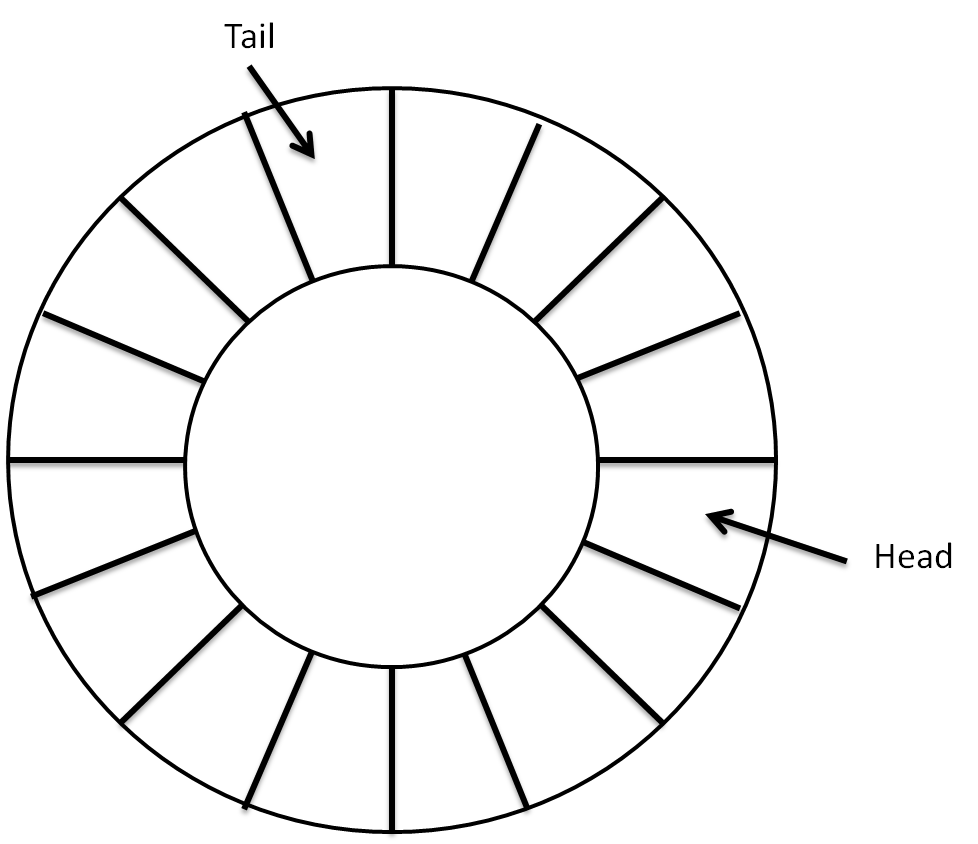
\includegraphics[scale=0.5]{img/ring-buffer.eps}
 \caption{The circular buffer.} \label{fig:circular-buffer}
\end{figure}

If we set a maximum size of the buffer instead of dynamically allocate 
memories, the queue can be defined with the below ANSI C code.

\lstset{language=C}
\begin{lstlisting}
struct Queue{
  Key* buf;
  int head, tail, size;
};
\end{lstlisting}

When initialize the queue, we are explicitly asked to provide the maximum
size as argument.

\begin{lstlisting}
struct Queue* createQ(int max){
  struct Queue* q = (struct Queue*)malloc(sizeof(struct Queue));
  q->buf = (Key*)malloc(sizeof(Key)*max);
  q->size = max;
  q->head = q->tail = 0;
  return q;
}
\end{lstlisting}

To test if a queue is empty is trivial.

\begin{algorithmic}
\Function{Empty?}{$Q$}
  \State \Return \Call{Head}{$Q$} = \Call{Tail}{$Q$}
\EndFunction
\end{algorithmic}

One brute-force implementation for \textproc{Enqueue} and \textproc{Dequeue}
is to calculate the modular of index blindly as the following.

\begin{algorithmic}
\Function{Enqueue}{$Q, x$}
  \If{$\lnot$ \Call{Full?}{$Q$}}
    \State \Call{Tail}{$Q$} $\gets $ (\Call{Tail}{$Q$} + 1) $\mod$ \Call{Size}{$Q$}
    \State \Call{Buffer}{$Q$}[\Call{Tail}{$Q$}] $\gets x$
  \EndIf
\EndFunction
\end{algorithmic}

\begin{algorithmic}
\Function{Head}{$Q$}
  \If{$\lnot$ \Call{Empty?}{$Q$}}
    \State \Return \Call{Buffer}{$Q$}[\Call{Head}{$Q$}]
  \EndIf
\EndFunction
\end{algorithmic}

\begin{algorithmic}
\Function{Dequeue}{$Q$}
  \If{$\lnot$ \Call{Empty?}{$Q$}}
    \State \Call{Head}{$Q$} $\gets $ (\Call{Head}{$Q$} + 1) $\mod$ \Call{Size}{$Q$}
  \EndIf
\EndFunction
\end{algorithmic}

However, modular is expensive and slow depends on some settings, so one
may replace it by some adjustment. For example as in the below ANSI C
program.

\begin{lstlisting}
void enQ(struct Queue* q, Key x){
  if(!fullQ(q)){
    q->buf[q->tail++] = x;
    q->tail -= q->tail< q->size ? 0 : q->size;
  }
}

Key headQ(struct Queue* q){
  return q->buf[q->head]; /* Assume queue isn't empty */
}

Key deQ(struct Queue* q){
  Key x = headQ(q);
  q->head++;
  q->head -= q->head< q->size ? 0 : q->size;
  return x;
}
\end{lstlisting}

\begin{Exercise}
As the circular buffer is allocated with a maximum size parameter, please
write a function to test if a queue is full to avoid overflow. Note
there are two cases, one is that the head is in front of the tail,
the other is on the contrary.
\end{Exercise}

% ================================================================
%                 the 1st version
% ================================================================
\section{Purely functional solution}

Chris Okasaki mentioned a simple and straightforward functional solution
in \cite{okasaki-book}. Observe that the singlely linked-list, which
is the backend data structure in most functional settings, performs 
well on head in constant $O(1)$ time, It only performs bad on tail, which
down-grades to linear $O(N)$ time, where $N$ is the length of the list.
One idea is to maintain two linked-lists as a queue. concatenate these
two lists in tail-to-tail manner. The shape of the queue looks like a 
horseshoe magnet as shown in figure \ref{fig:horseshoe-magnet}.

\begin{figure}[htbp]
  \centering
  \setlength{\unitlength}{1cm}
  \begin{picture}(10, 5)
  \put(0, 0){\line(1, 0){5}}
  \put(0, 0){\line(0, 1){1}}
  \put(0, 1){\line(1, 0){5}}

  \put(0, 5){\line(1, 0){5}}
  \put(0, 4){\line(0, 1){1}}
  \put(0, 4){\line(1, 0){5}}

  \put(5, 2.5){\oval(7, 5)[r]}
  \put(5, 2.5){\oval(5, 3)[r]}
  \end{picture}
  \caption{A queue with front and rear list shapes like a horseshoe magnet.} \label{fig:horseshoe-magnet}
\end{figure}

% ================================================================
%                 Short summary
% ================================================================
\section{Notes and short summary}

TODO: Mention the priority queues, which can be realized by using heap.

% ================================================================
%                 Appendix
% ================================================================

\begin{thebibliography}{99}

\bibitem{PODC96}
Maged M. Michael and Michael L. Scott. ``Simple, Fast, and Practical Non-Blocking and Blocking Concurrent Queue Algorithms''. http://www.cs.rochester.edu/research/synchronization/pseudocode/queues.html

\bibitem{SutterDDJ}
Herb Sutter. ``Writing a Generalized Concurrent Queue''. Dr. Dobb's Oct 29, 2008. http://drdobbs.com/cpp/211601363?pgno=1

\bibitem{CLRS}
Thomas H. Cormen, Charles E. Leiserson, Ronald L. Rivest and Clifford Stein. ``Introduction to Algorithms, Second Edition''. The MIT Press, 2001. ISBN: 0262032937.

\bibitem{okasaki-book}
Chris Okasaki. ``Purely Functional Data Structures''. Cambridge university press, (July 1, 1999), ISBN-13: 978-0521663502

\end{thebibliography}

\ifx\wholebook\relax \else
\end{document}
\fi
